% =============================================================================
%  Diplomado en Data Science Aplicada con Python para la Toma de Decisiones
%  Clase 28: Modelos en Producci\'on + Segmentaci\'on para Conteo
%  Arca Continental Ecuador | UDLA
%  Compilar: pdflatex -shell-escape presentacion.tex (x2 para refs)
% =============================================================================
\documentclass[aspectratio=169, 11pt]{beamer}

\usepackage[T1]{fontenc}
\usepackage[utf8]{inputenc}
\usepackage[spanish,es-noshorthands]{babel}
\usepackage{FiraSans}
\usepackage{FiraMono}
\renewcommand{\familydefault}{\sfdefault}
\usepackage{graphicx}
\usepackage{tikz}
\usetikzlibrary{arrows.meta, positioning, shapes.geometric, shapes.misc,
  calc, fit, decorations.pathreplacing, backgrounds}
\usepackage{fontawesome5}
\usepackage{minted}
\usepackage{tcolorbox}
\tcbuselibrary{minted, skins, breakable}
\usepackage{booktabs}
\usepackage{colortbl}
\usepackage{multicol}
\usepackage{hyperref}
\usepackage{calc}
\usepackage{amsmath}

\definecolor{arcaRed}{HTML}{C82B40}
\definecolor{arcaDark}{HTML}{6B1525}
\definecolor{udlaCrimson}{HTML}{A31545}
\definecolor{arcaGray}{HTML}{F5F5F5}
\definecolor{arcaLightGray}{HTML}{EBEBEB}
\definecolor{textDark}{HTML}{2D2D2D}
\definecolor{textMuted}{HTML}{6B7280}
\definecolor{codeGreen}{HTML}{16A34A}
\definecolor{codeBlue}{HTML}{2563EB}
\definecolor{codeOrange}{HTML}{EA580C}
\definecolor{codePurple}{HTML}{7C3AED}

\usetheme{default}
\usecolortheme{default}
\setbeamertemplate{navigation symbols}{}
\setbeamertemplate{footline}{}
\setbeamertemplate{headline}{}
\setbeamercolor{normal text}{fg=textDark}
\setbeamercolor{frametitle}{fg=arcaRed, bg=white}
\setbeamercolor{title}{fg=white}
\setbeamercolor{subtitle}{fg=white!85}
\setbeamercolor{author}{fg=white!80}
\setbeamercolor{date}{fg=white!70}
\setbeamercolor{item}{fg=arcaRed}
\setbeamercolor{subitem}{fg=arcaDark}
\setbeamercolor{block title}{fg=white, bg=arcaRed}
\setbeamercolor{block body}{fg=textDark, bg=arcaGray}
\setbeamercolor{section in toc}{fg=arcaDark}
\setbeamerfont{frametitle}{size=\Large, series=\bfseries}
\setbeamerfont{title}{size=\huge, series=\bfseries}
\setbeamerfont{subtitle}{size=\large}
\setbeamerfont{author}{size=\normalsize}
\setbeamerfont{date}{size=\small}
\setbeamerfont{block title}{size=\normalsize, series=\bfseries}
\setbeamerfont{footnote}{size=\tiny}
\setbeamertemplate{itemize item}{\scriptsize\raise1.5pt\hbox{\color{arcaRed}$\blacktriangleright$}}
\setbeamertemplate{itemize subitem}{\scriptsize\raise1pt\hbox{\color{arcaDark}$\bullet$}}
\setbeamertemplate{enumerate items}[default]
\setbeamercolor{enumerate item}{fg=arcaRed}

\setbeamertemplate{headline}{%
  \begin{tikzpicture}[remember picture, overlay]
    \fill[arcaDark] (current page.north west) rectangle
      ([yshift=-0.7cm]current page.north east);
    \node[anchor=west, inner sep=0pt] at
      ([xshift=0.6cm, yshift=-0.35cm]current page.north west)
      {
\includegraphics[height=0.45cm]{../logo_udla_white.png}};
    \node[anchor=east, inner sep=0pt] at
      ([xshift=-0.6cm, yshift=-0.35cm]current page.north east)
      {
\includegraphics[height=0.45cm]{../ArcaContinental_white.png}};
  \end{tikzpicture}%
  \vspace{0.7cm}%
}

\setbeamertemplate{footline}{%
  \begin{tikzpicture}[remember picture, overlay]
    \node[anchor=south east, font=\scriptsize\bfseries\color{arcaRed}] at
      ([xshift=-0.5cm, yshift=0.15cm]current page.south east)
      {\insertframenumber};
  \end{tikzpicture}%
  \vspace{0.3cm}%
}

\setbeamertemplate{frametitle}{%
  \vspace{0.25cm}%
  \usebeamerfont{frametitle}\usebeamercolor[fg]{frametitle}\insertframetitle%
  \par\vspace{2pt}%
  \begin{tikzpicture}
    \fill[arcaRed] (0,0) rectangle (3cm, 1.5pt);
    \fill[arcaLightGray] (3cm,0) rectangle (\textwidth, 0.5pt);
  \end{tikzpicture}%
  \vspace{0.1cm}%
}

\newtcblisting{pyblock}[1][]{%
  listing engine=minted, minted language=python, minted style=friendly,
  minted options={fontsize=\small, linenos=false, breaklines=true, python3=true},
  colback=arcaGray, colframe=arcaRed, left=4pt, right=4pt, top=4pt, bottom=4pt,
  boxrule=0pt, leftrule=3pt, arc=2pt, listing only, #1}

\newcommand{\sectionframe}[2]{%
  \begingroup
  \setbeamertemplate{headline}{}%
  \setbeamertemplate{footline}{}%
  \begin{frame}[plain, noframenumbering]
    \begin{tikzpicture}[remember picture, overlay]
      \fill[arcaRed] (current page.south west) rectangle (current page.north east);
      \node[anchor=center, text=white, font=\Huge\bfseries, text width=12cm,
            align=center] at ([yshift=0.5cm]current page.center) {#1};
      \node[anchor=center, text=white!80, font=\large, text width=10cm,
            align=center] at ([yshift=-0.8cm]current page.center) {#2};
    \end{tikzpicture}
  \end{frame}
  \endgroup
}

\title{Diplomado en Data Science Aplicada\\con Python para la Toma de Decisiones}
\subtitle{Clase 28: Modelos en Producci\'on + Segmentaci\'on para Conteo}
\author{Carlos Enrique Mosquera Trujillo}
\date{15 de Mayo, 2026}

\begin{document}

% ── PORTADA ──────────────────────────────────────────────────────────────────
{
\setbeamertemplate{headline}{}
\setbeamertemplate{footline}{}
\begin{frame}[plain, noframenumbering]
  \begin{tikzpicture}[remember picture, overlay]
    \fill[arcaDark] (current page.south west) rectangle (current page.north east);
    \fill[arcaRed] ([yshift=-3.5cm]current page.north west) rectangle
      ([yshift=-4.2cm]current page.north east);
    \node[anchor=west, inner sep=0pt] at
      ([xshift=1cm, yshift=-1.5cm]current page.north west)
      {
\includegraphics[height=1cm]{../logo_udla_white.png}};
    \node[anchor=east, inner sep=0pt] at
      ([xshift=-1cm, yshift=-1.5cm]current page.north east)
      {
\includegraphics[height=1cm]{../ArcaContinental_white.png}};
  \end{tikzpicture}
  \vspace{2.5cm}
  \begin{center}
    {\usebeamerfont{title}\usebeamercolor[fg]{title}\inserttitle\par}
    \vspace{0.4cm}
    {\usebeamerfont{subtitle}\usebeamercolor[fg]{subtitle}\insertsubtitle\par}
    \vspace{0.6cm}
    {\usebeamerfont{author}\usebeamercolor[fg]{author}\insertauthor\par}
    \vspace{0.15cm}
    {\usebeamerfont{date}\usebeamercolor[fg]{date}\insertdate\par}
  \end{center}
\end{frame}
}

% ── HOJA DE RUTA ─────────────────────────────────────────────────────────────
\begin{frame}[shrink]{Hoja de Ruta de Hoy}
  \vspace{4pt}
  \begin{center}
  \begin{tikzpicture}[
    node distance=0.25cm,
    roadstep/.style={rectangle, rounded corners=4pt, draw=arcaRed, fill=arcaRed!8,
                 minimum width=11.5cm, minimum height=0.55cm,
                 font=\footnotesize\bfseries\color{arcaDark}, align=left,
                 text width=10.5cm, inner sep=4pt},
    num/.style={circle, fill=arcaRed, text=white, font=\scriptsize\bfseries,
                minimum size=0.45cm, inner sep=0pt},
  ]
    \node[roadstep] (s0) {\hspace{0.7cm}Cierre clase 27: entrenar el detector de tumores cerebrales};
    \node[roadstep, below=of s0] (s1) {\hspace{0.7cm}M\'etricas a profundidad: cu\'al escoger seg\'un el dominio};
    \node[roadstep, below=of s1] (s2) {\hspace{0.7cm}Guardar y cargar el modelo (\texttt{best.pt}, ONNX, versionado)};
    \node[roadstep, below=of s2] (s3) {\hspace{0.7cm}Segmentaci\'on: por qu\'e, cu\'ando, qu\'e devuelve};
    \node[roadstep, below=of s3] (s4) {\hspace{0.7cm}API de YOLO segmentation: \texttt{masks.data}, \texttt{.xy}, \texttt{.xyn}, \'area};
    \node[roadstep, below=of s4] (s5) {\hspace{0.7cm}Las 80 clases COCO de seg: qu\'e reconoce sin entrenar};
    \node[roadstep, below=of s5] (s6) {\hspace{0.7cm}\textbf{Caso negocio:} contar p\'ildoras (Roboflow $\to$ LS $\to$ entrenar)};
    \node[roadstep, below=of s6] (s7) {\hspace{0.7cm}\textbf{App Gradio:} cont\'on de p\'ildoras como producto final};

    \foreach \i in {0,...,7}{
      \node[num] at ([xshift=0.4cm]s\i.west) {\the\numexpr\i+1};
    }
  \end{tikzpicture}
  \end{center}
\end{frame}

\begin{frame}[shrink]{Hero: las Dos Mitades de Hoy}
  \vspace{2pt}
  \begin{center}
    
\includegraphics[width=0.97\textwidth]{fig_hero.png}
  \end{center}

  \vspace{2pt}
  {\scriptsize\color{textMuted}
    \faLightbulb\hspace{4pt} Primera mitad: cerrar la cl\'inica (brain tumor).
    Segunda mitad: abrir la farmac\'eutica (p\'ildoras). Una clase, dos
    problemas, mismo stack.}
\end{frame}

% =============================================================================
%  BLOQUE 1: CIERRE BRAIN TUMOR
% =============================================================================
\sectionframe{Cierre Clase 27}{Entrenar el detector de tumores cerebrales}

\begin{frame}[shrink]{Recordatorio: D\'onde Quedamos}
  \vspace{6pt}
  {\footnotesize\color{arcaDark}\bfseries
    En la clase 27 hicimos el etiquetado en Label Studio. Hoy bajamos las
    etiquetas y entrenamos. Mismo c\'odigo que usamos para placas.}

  \vspace{14pt}
  {\footnotesize
  \begin{itemize}\setlength{\itemsep}{6pt}
    \item[{\color{arcaRed}\scriptsize\faArrowRight}]
      Dataset: \texttt{brain-tumor} de Ultralytics, 893 train + 223 val MRI.
    \item[{\color{arcaRed}\scriptsize\faArrowRight}]
      2 clases: \texttt{negative} (no tumor) y \texttt{positive} (tumor).
    \item[{\color{arcaRed}\scriptsize\faArrowRight}]
      80\% pre-etiquetado con ground truth real, 20\% etiquetado por el
      equipo (sin ser radi\'ologos).
    \item[{\color{codeGreen}\scriptsize\faArrowRight}]
      Pregunta clave: \emph{?`qu\'e m\'etrica miramos?}
  \end{itemize}
  }
\end{frame}

\begin{frame}[fragile,shrink]{C\'odigo: Bajar y Entrenar}
  \vspace{-4pt}
  \begin{pyblock}
# Bajar (mismo flow que clase 27)
brain_dir = export_labels(ID_BRAIN, "brain.zip", "brain")
fetch_ls_images(ID_BRAIN, brain_dir / "images_raw")
organize_yolo(brain_dir)

# Entrenar
from ultralytics import YOLO
model_b = YOLO("yolo26n.pt")
results_b = model_b.train(
    data=str(yaml_path_brain),
    epochs=20,
    imgsz=640,
    batch=16,
    device="cuda",
    project="runs", name="brain", exist_ok=True,
)
  \end{pyblock}
\end{frame}

% =============================================================================
%  BLOQUE 2: METRICAS
% =============================================================================
\sectionframe{M\'etricas a Profundidad}{Cu\'al escoger depende del dominio, no del modelo}

\begin{frame}[shrink]{Las 5 M\'etricas que YOLO Reporta}
  \vspace{8pt}
  {\footnotesize
  \begin{tabular}{@{}p{3.0cm} p{4.0cm} p{5.0cm}@{}}
    \toprule
    \textbf{M\'etrica} & \textbf{F\'ormula} & \textbf{Qu\'e mide} \\
    \midrule
    \rowcolor{arcaGray}
    \textbf{Precision}
    & TP / (TP + FP)
    & De lo que detect\'e, ?`qu\'e \% era real? \\
    \textbf{Recall}
    & TP / (TP + FN)
    & De lo real, ?`qu\'e \% detect\'e? \\
    \rowcolor{arcaGray}
    \textbf{F1}
    & 2$\cdot$P$\cdot$R / (P+R)
    & Media arm\'onica. Equilibra ambos. \\
    \textbf{mAP@0.5}
    & AP a IoU $\geq$ 0.5
    & "Cajas suficientemente bien" \\
    \rowcolor{arcaGray}
    \textbf{mAP@0.5:0.95}
    & AP promedio en 10 umbrales
    & Cajas BIEN alineadas (m\'as estricto) \\
    \bottomrule
  \end{tabular}
  }

  \vspace{10pt}
  \begin{tcolorbox}[colback=arcaGray, colframe=arcaRed, boxrule=0.5pt,
    arc=2pt, left=6pt, right=6pt, top=4pt, bottom=4pt]
    {\scriptsize\color{arcaDark}
    \faKey\hspace{4pt} \textbf{mAP} = \emph{mean Average Precision}.
    \'Area bajo la curva precision--recall, promediada entre clases.
    Es la m\'etrica est\'andar en detection y segmentation.}
  \end{tcolorbox}
\end{frame}

\begin{frame}[shrink]{Precision vs Recall: el Dominio Manda}
  \vspace{4pt}
  \begin{center}
    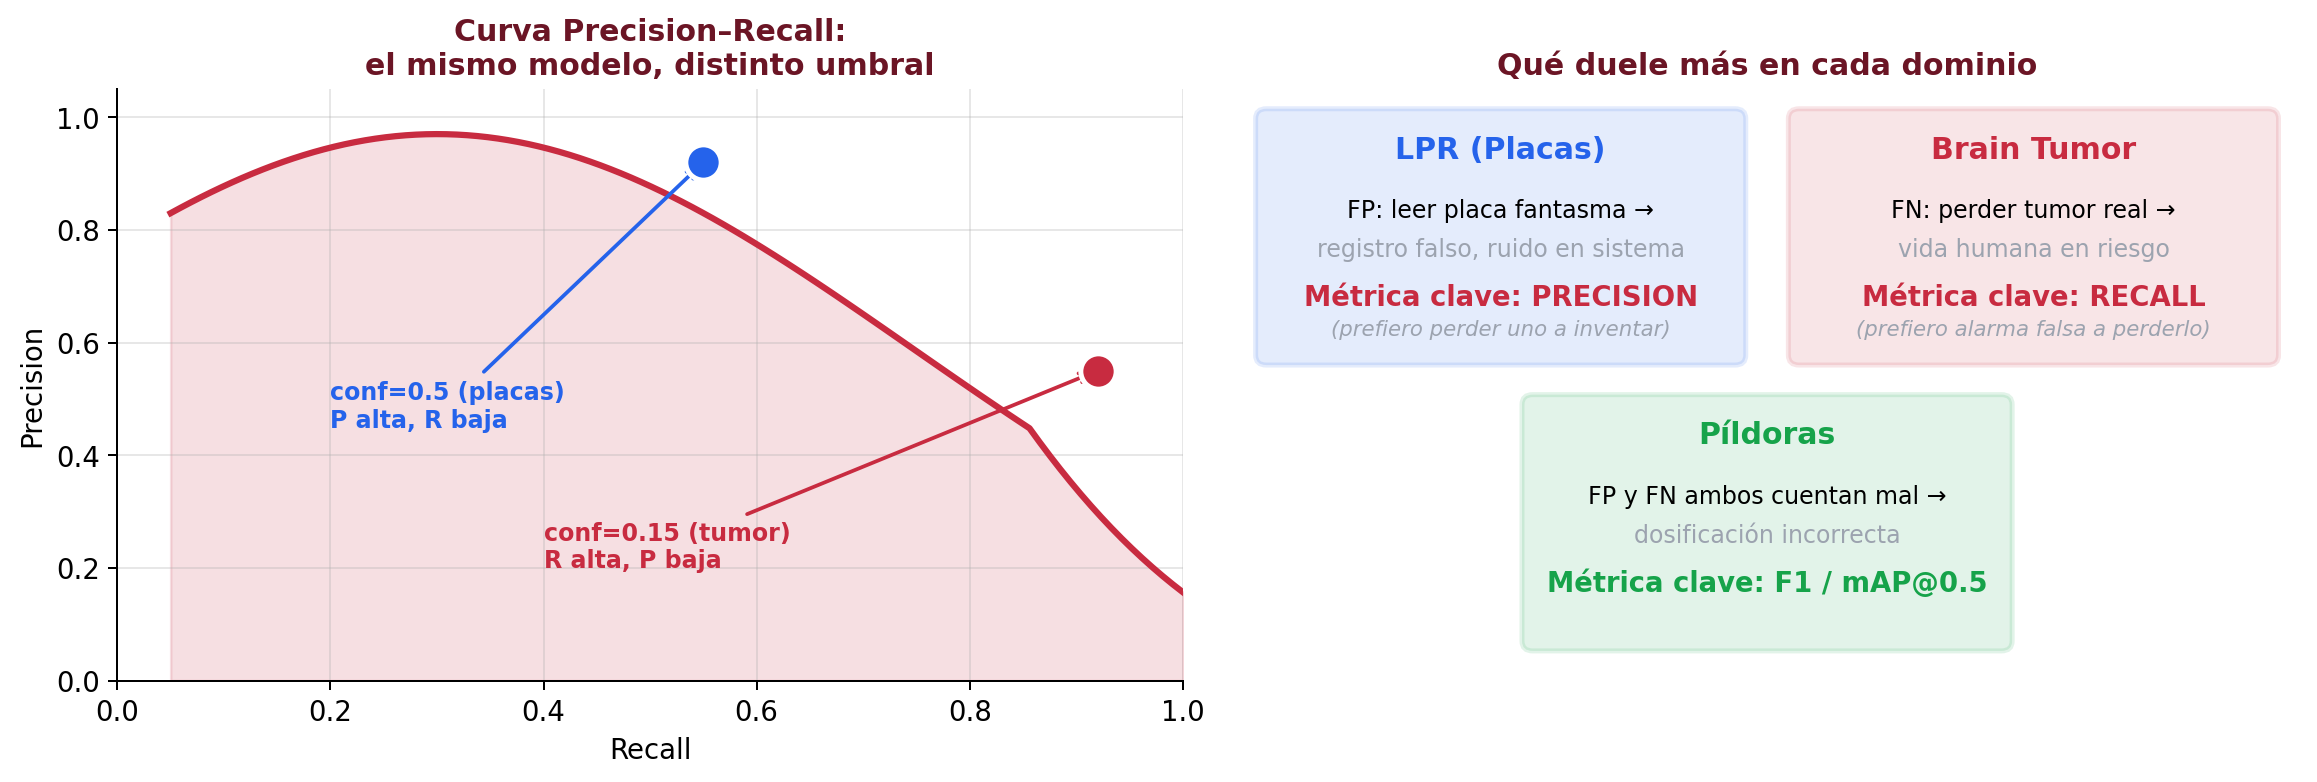
\includegraphics[width=0.97\textwidth]{fig_precision_recall.png}
  \end{center}

  \vspace{2pt}
  {\scriptsize\color{textMuted}
    \faLightbulb\hspace{4pt} El mismo modelo da m\'etricas distintas seg\'un el
    \texttt{conf} threshold. La decisi\'on no es t\'ecnica, es de negocio: ?`qu\'e
    duele m\'as, un falso positivo o un falso negativo?}
\end{frame}

\begin{frame}[shrink]{mAP@0.5 vs mAP@0.5:0.95}
  \vspace{4pt}
  \begin{center}
    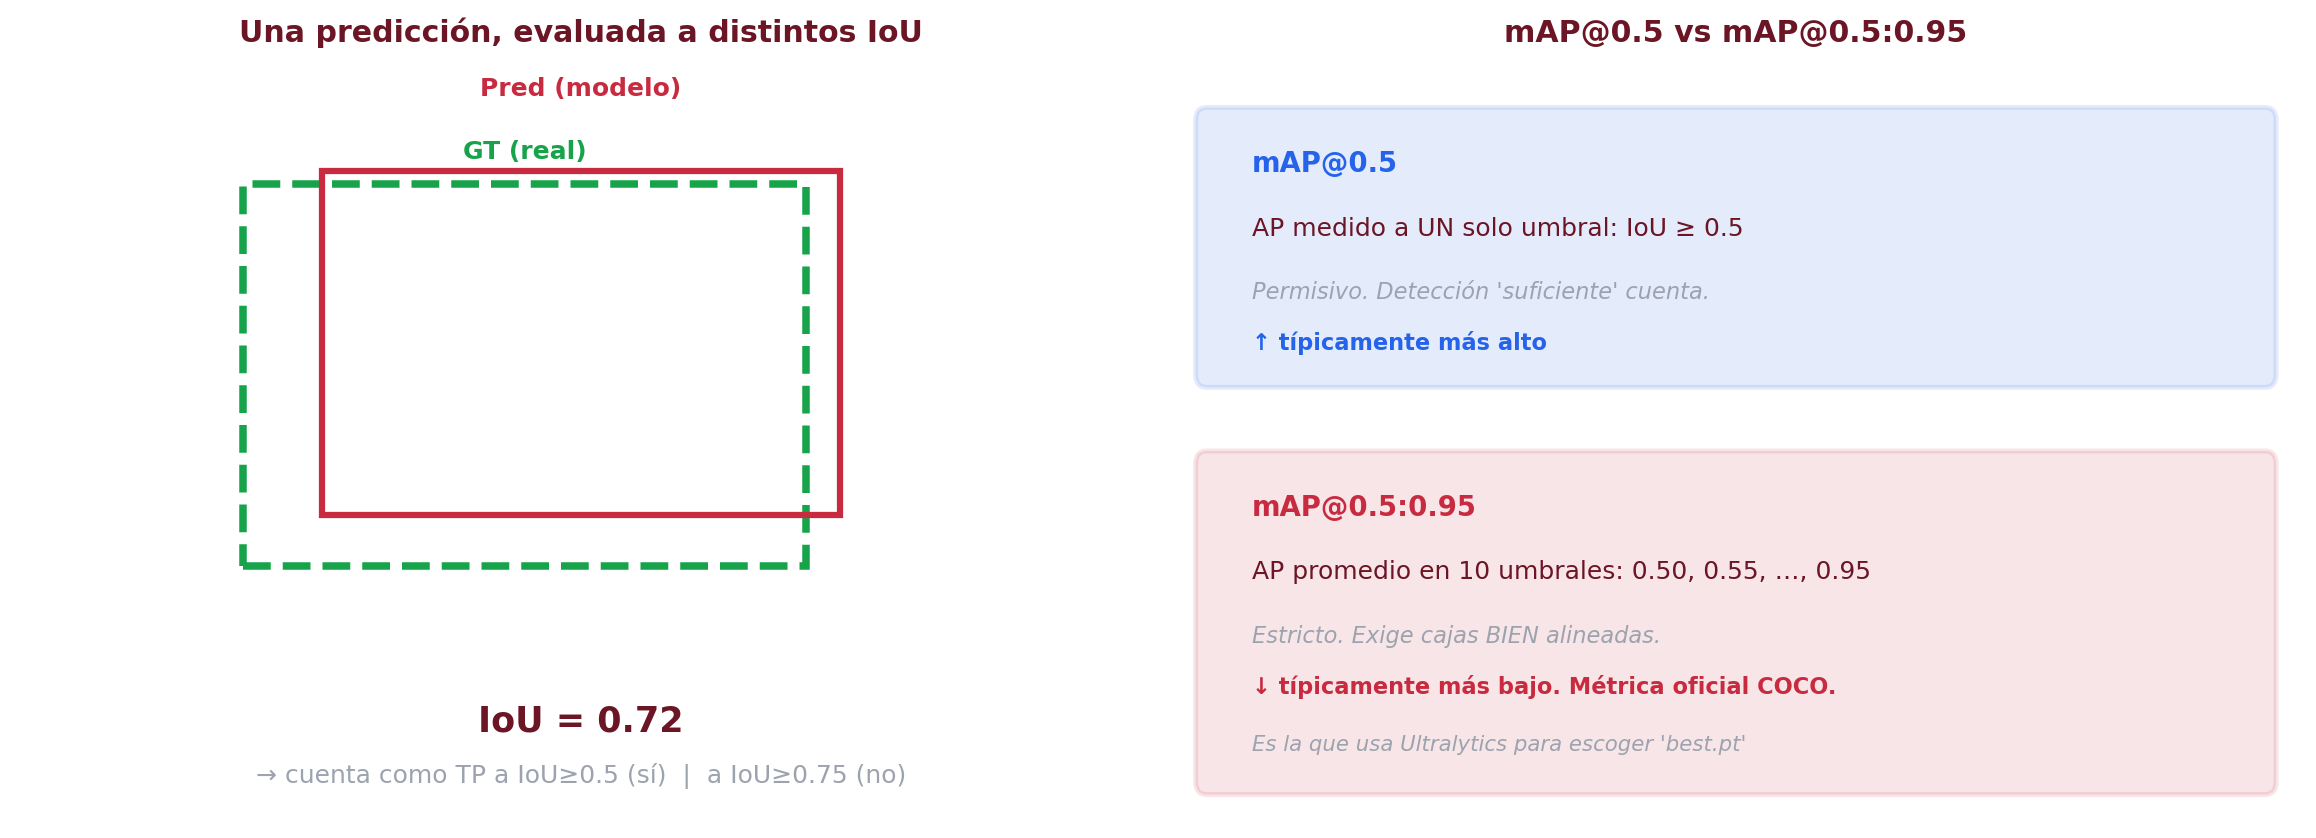
\includegraphics[width=0.97\textwidth]{fig_map_thresholds.png}
  \end{center}

  \vspace{2pt}
  {\scriptsize\color{textMuted}
    \faLightbulb\hspace{4pt} Ultralytics elige \texttt{best.pt} usando
    mAP@0.5:0.95 (la estricta). En reportes ejecutivos suele mostrarse
    mAP@0.5 porque "se ve mejor". Saber esto te evita comparar peras con manzanas.}
\end{frame}

\begin{frame}[shrink]{El \texttt{conf} Threshold es un Slider}
  \vspace{2pt}
  \begin{center}
    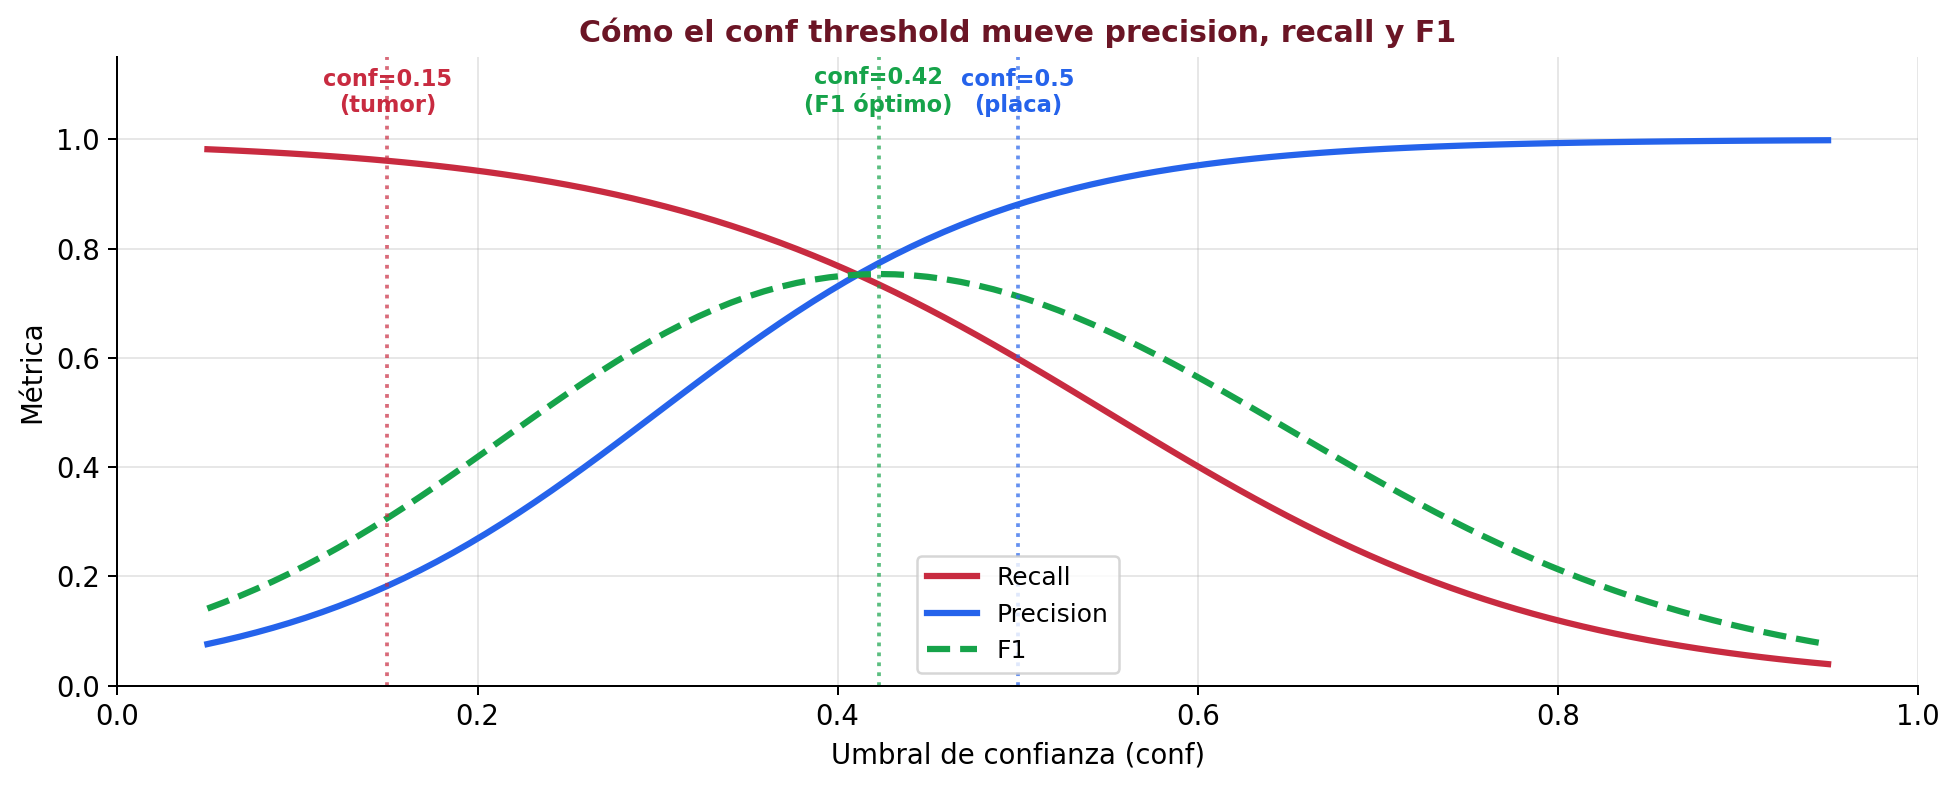
\includegraphics[width=0.95\textwidth]{fig_conf_slider.png}
  \end{center}

  \vspace{2pt}
  {\scriptsize\color{textMuted}
    \faLightbulb\hspace{4pt} Para subir recall: bajar \texttt{conf}. Para subir
    precision: subir \texttt{conf}. El modelo no cambia; cambia tu tolerancia al ruido.}
\end{frame}

\begin{frame}[shrink]{Leer la Confusion Matrix}
  \vspace{2pt}
  \begin{center}
    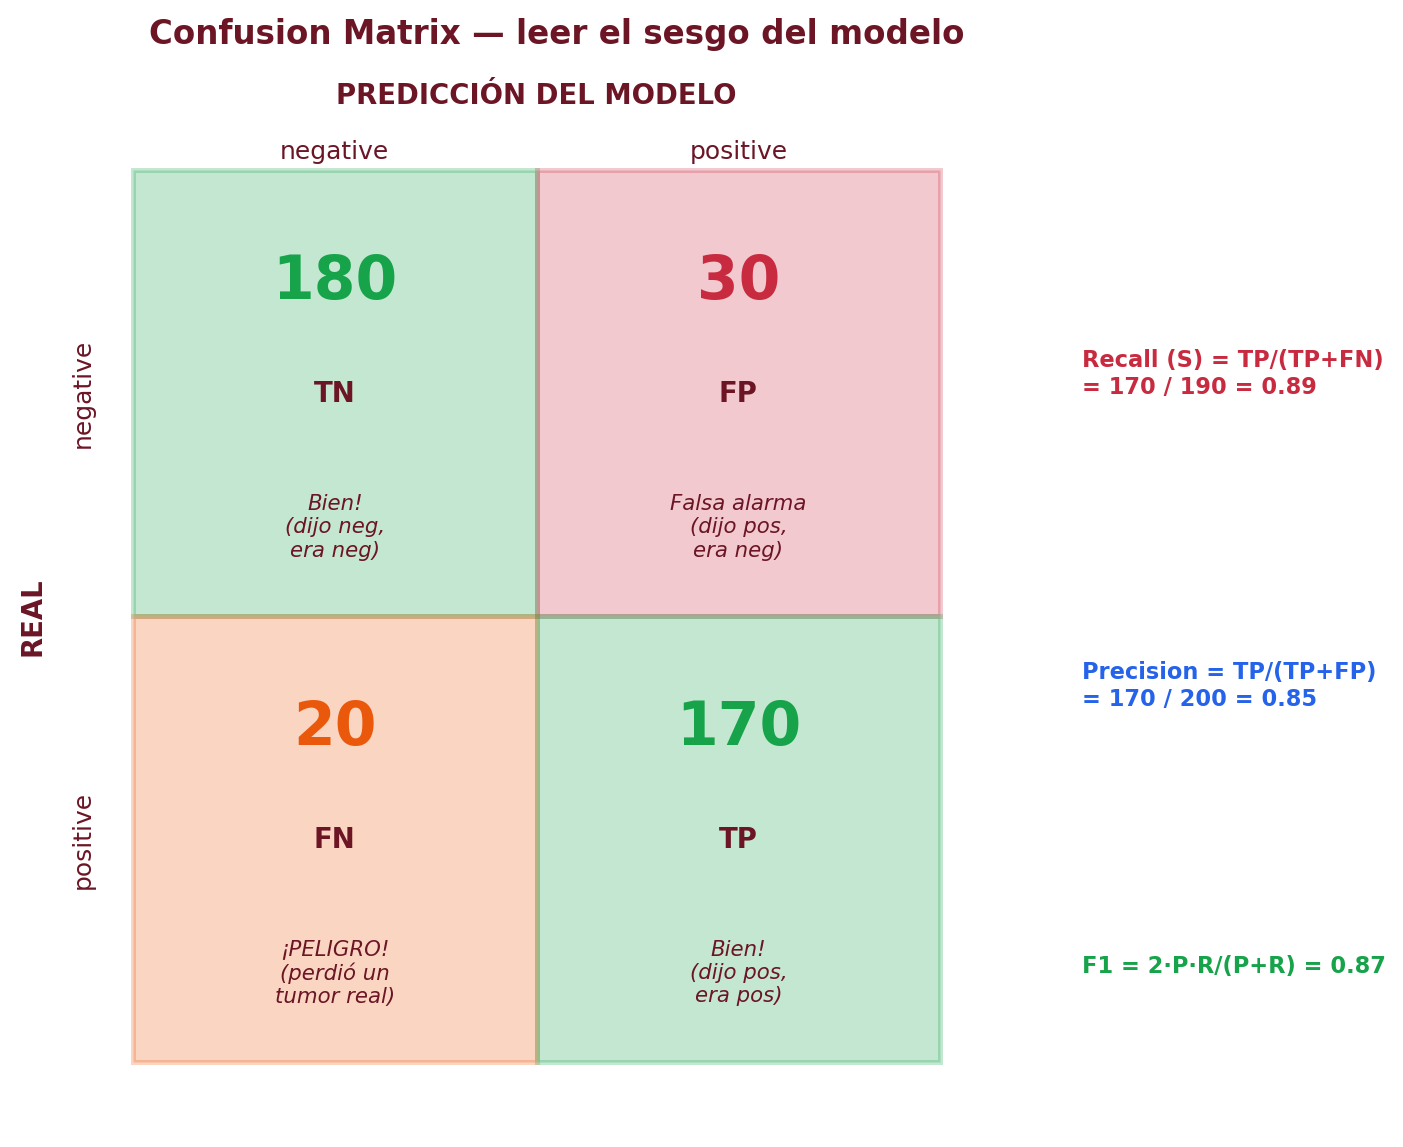
\includegraphics[width=0.62\textwidth]{fig_confusion.png}
  \end{center}

  \vspace{2pt}
  {\scriptsize\color{textMuted}
    \faLightbulb\hspace{4pt} En brain tumor el cuadrante FN (perder un tumor
    real) es el m\'as caro. Un mAP alto puede esconderlo: \emph{siempre} mirar
    la confusi\'on con un experto del dominio.}
\end{frame}

% =============================================================================
%  BLOQUE 3: GUARDAR Y CARGAR
% =============================================================================
\sectionframe{Guardar y Cargar el Modelo}{De \texttt{runs/} a producci\'on}

\begin{frame}[shrink]{El Recorrido de un Modelo}
  \vspace{2pt}
  \begin{center}
    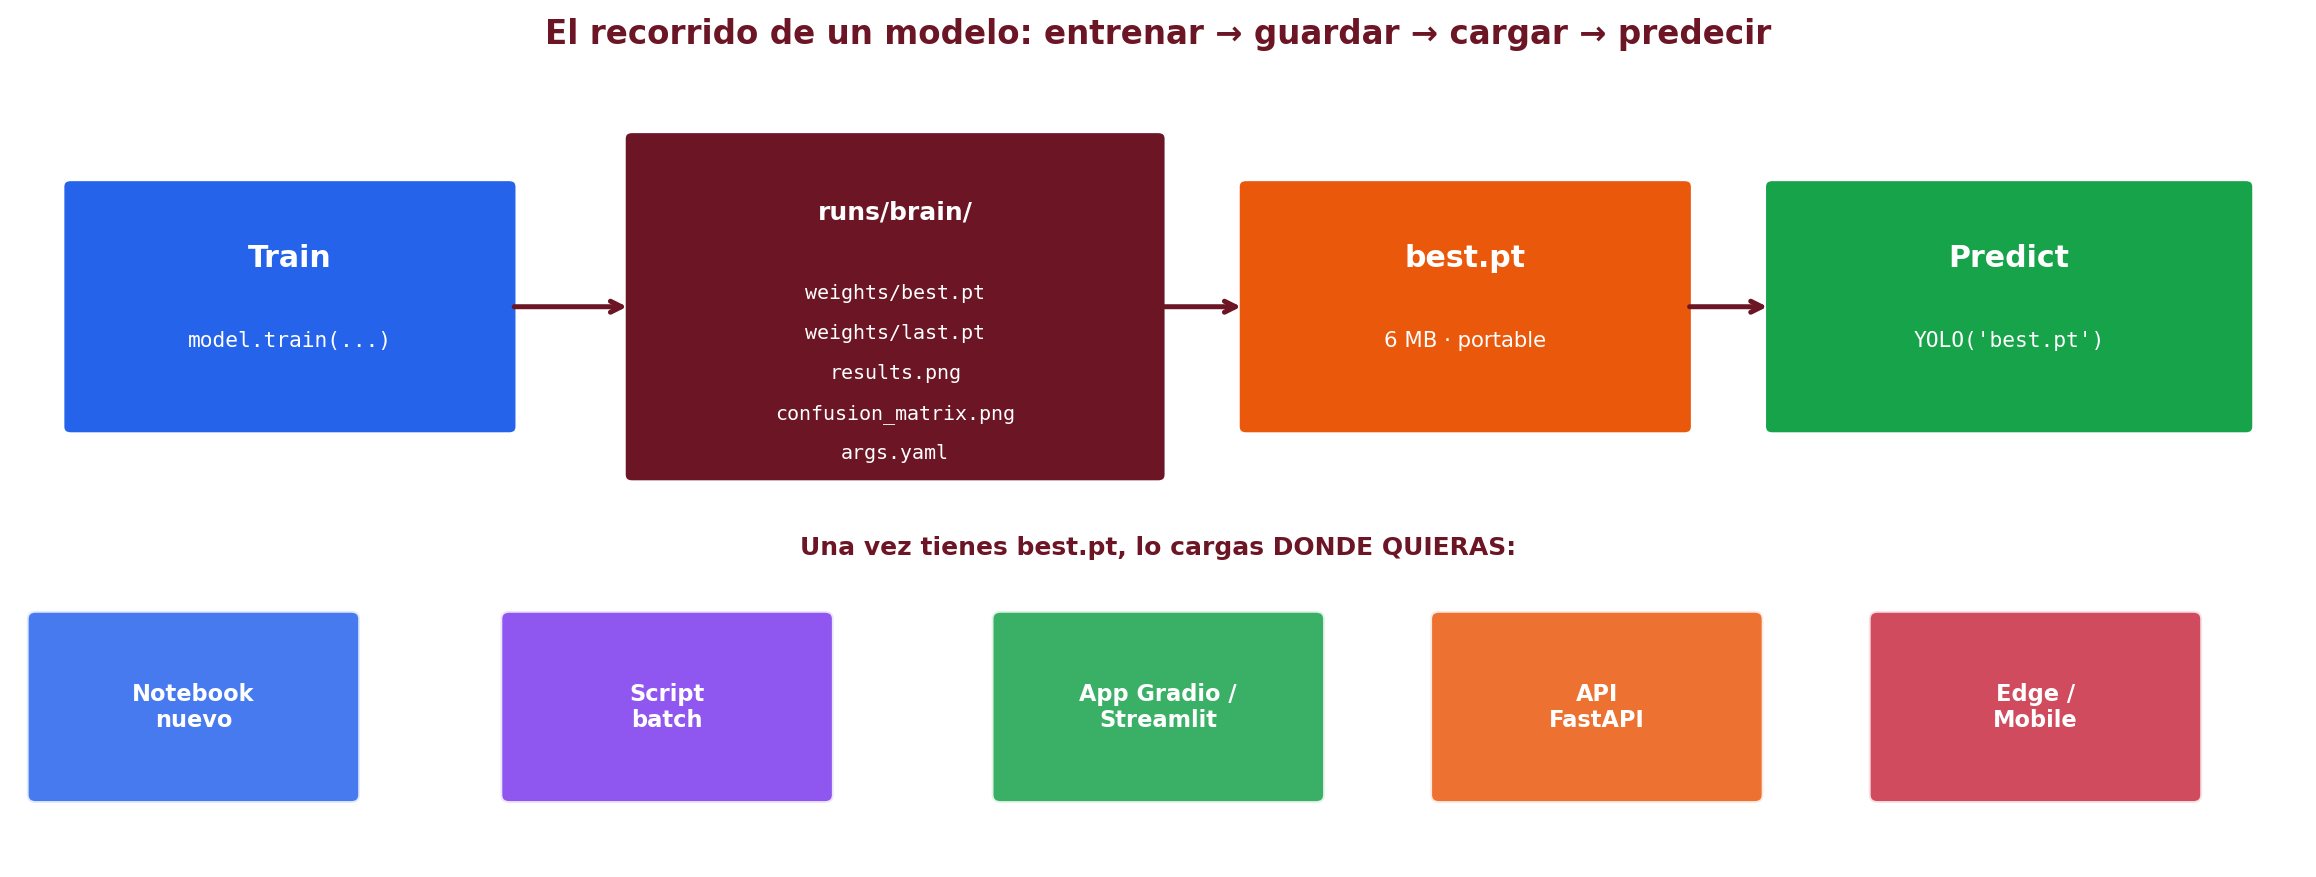
\includegraphics[width=0.97\textwidth]{fig_save_load.png}
  \end{center}

  \vspace{2pt}
  {\scriptsize\color{textMuted}
    \faLightbulb\hspace{4pt} El \emph{\'unico} archivo que necesitas para
    predecir en otro contexto es \texttt{best.pt} ($\sim$6 MB). Todo lo dem\'as
    (curvas, logs, last.pt) es debugging.}
\end{frame}

\begin{frame}[fragile,shrink]{Versionado Simple --- el Patr\'on que Funciona}
  \vspace{-4pt}
  \begin{pyblock}
# Convencion: tarea_arquitectura_fecha.pt
import datetime
today = datetime.date.today().isoformat()

models_dir = Path("models")
models_dir.mkdir(exist_ok=True)
shutil.copy(
    "runs/brain/weights/best.pt",
    models_dir / f"brain_yolo26n_{today}.pt"
)

# En otro lugar (otro Colab, otra maquina, otro servidor):
modelo = YOLO("models/brain_yolo26n_2026-05-15.pt")
results = modelo("paciente_43.jpg", conf=0.15)
  \end{pyblock}

  \vspace{6pt}
  \begin{tcolorbox}[colback=codeGreen!8, colframe=codeGreen, boxrule=0.5pt,
    arc=2pt, left=6pt, right=6pt, top=4pt, bottom=4pt]
    {\scriptsize\color{arcaDark}
    \faKey\hspace{4pt}\textbf{Regla:} nunca sobreescribir. Cada
    re-entrenamiento es un archivo nuevo. Crecimiento: MLflow / W\&B
    cuando tengas docenas de modelos.}
  \end{tcolorbox}
\end{frame}

\begin{frame}[fragile,shrink]{Export ONNX: Sacarlo de Python}
  \vspace{-4pt}
  \begin{pyblock}
# Una vez fine-tuneado, exportar para deploy donde no haya Python:
model.export(format="onnx")        # universal: C++, Java, JavaScript
model.export(format="tflite")      # movil Android
model.export(format="coreml")      # iOS / macOS
model.export(format="engine")      # TensorRT (Jetson, 60+ FPS)

# Cada uno se carga distinto en su destino:
#   ONNX:    onnxruntime.InferenceSession("best.onnx")
#   TFLite:  tflite.Interpreter(model_path="best.tflite")
  \end{pyblock}

  \vspace{4pt}
  {\scriptsize\color{textMuted}
    \faLightbulb\hspace{4pt} Para producci\'on: \textbf{ONNX} es el formato
    m\'as portable. Lo levantas en un microservicio sin instalar PyTorch.}
\end{frame}

% =============================================================================
%  BLOQUE 4: SEGMENTACION
% =============================================================================
\sectionframe{Segmentaci\'on}{Cuando contar y medir importan, los bboxes no alcanzan}

\begin{frame}[shrink]{Detection vs Segmentation: Trade-offs}
  \vspace{8pt}
  {\footnotesize
  \begin{tabular}{@{}p{3.0cm} p{4.0cm} p{5.0cm}@{}}
    \toprule
    & \textbf{Detection (bbox)} & \textbf{Segmentation (mask)} \\
    \midrule
    \rowcolor{arcaGray}
    Output por objeto
    & 4 n\'umeros [x, y, w, h]
    & Pol\'igono ($\sim$20 puntos) \\
    Etiquetar
    & R\'apido (4 clicks)
    & 5--10$\times$ m\'as lento \\
    \rowcolor{arcaGray}
    Tama\~no de modelo
    & yolo26n: 6 MB
    & yolo26n-seg: 7 MB \\
    Velocidad inferencia
    & R\'apido
    & 10--20\% m\'as lento \\
    \rowcolor{arcaGray}
    Precisi\'on en densidad
    & Cae con solape
    & \textbf{Mantiene precisi\'on} \\
    Conteo exacto
    & Falla con NMS agresivo
    & \textbf{Conteo robusto} \\
    \bottomrule
  \end{tabular}
  }

  \vspace{10pt}
  \begin{tcolorbox}[colback=codeGreen!8, colframe=codeGreen, boxrule=0.5pt,
    arc=2pt, left=6pt, right=6pt, top=4pt, bottom=4pt]
    {\scriptsize\color{arcaDark}
    \faKey\hspace{4pt}\textbf{Regla pr\'actica:} si \emph{conteo} o \emph{\'area}
    importan, usar segmentation. Si solo importa \emph{est\'a o no est\'a},
    detection alcanza.}
  \end{tcolorbox}
\end{frame}

\begin{frame}[shrink]{Por Qu\'e P\'ildoras Necesitan Segmentaci\'on}
  \vspace{4pt}
  \begin{center}
    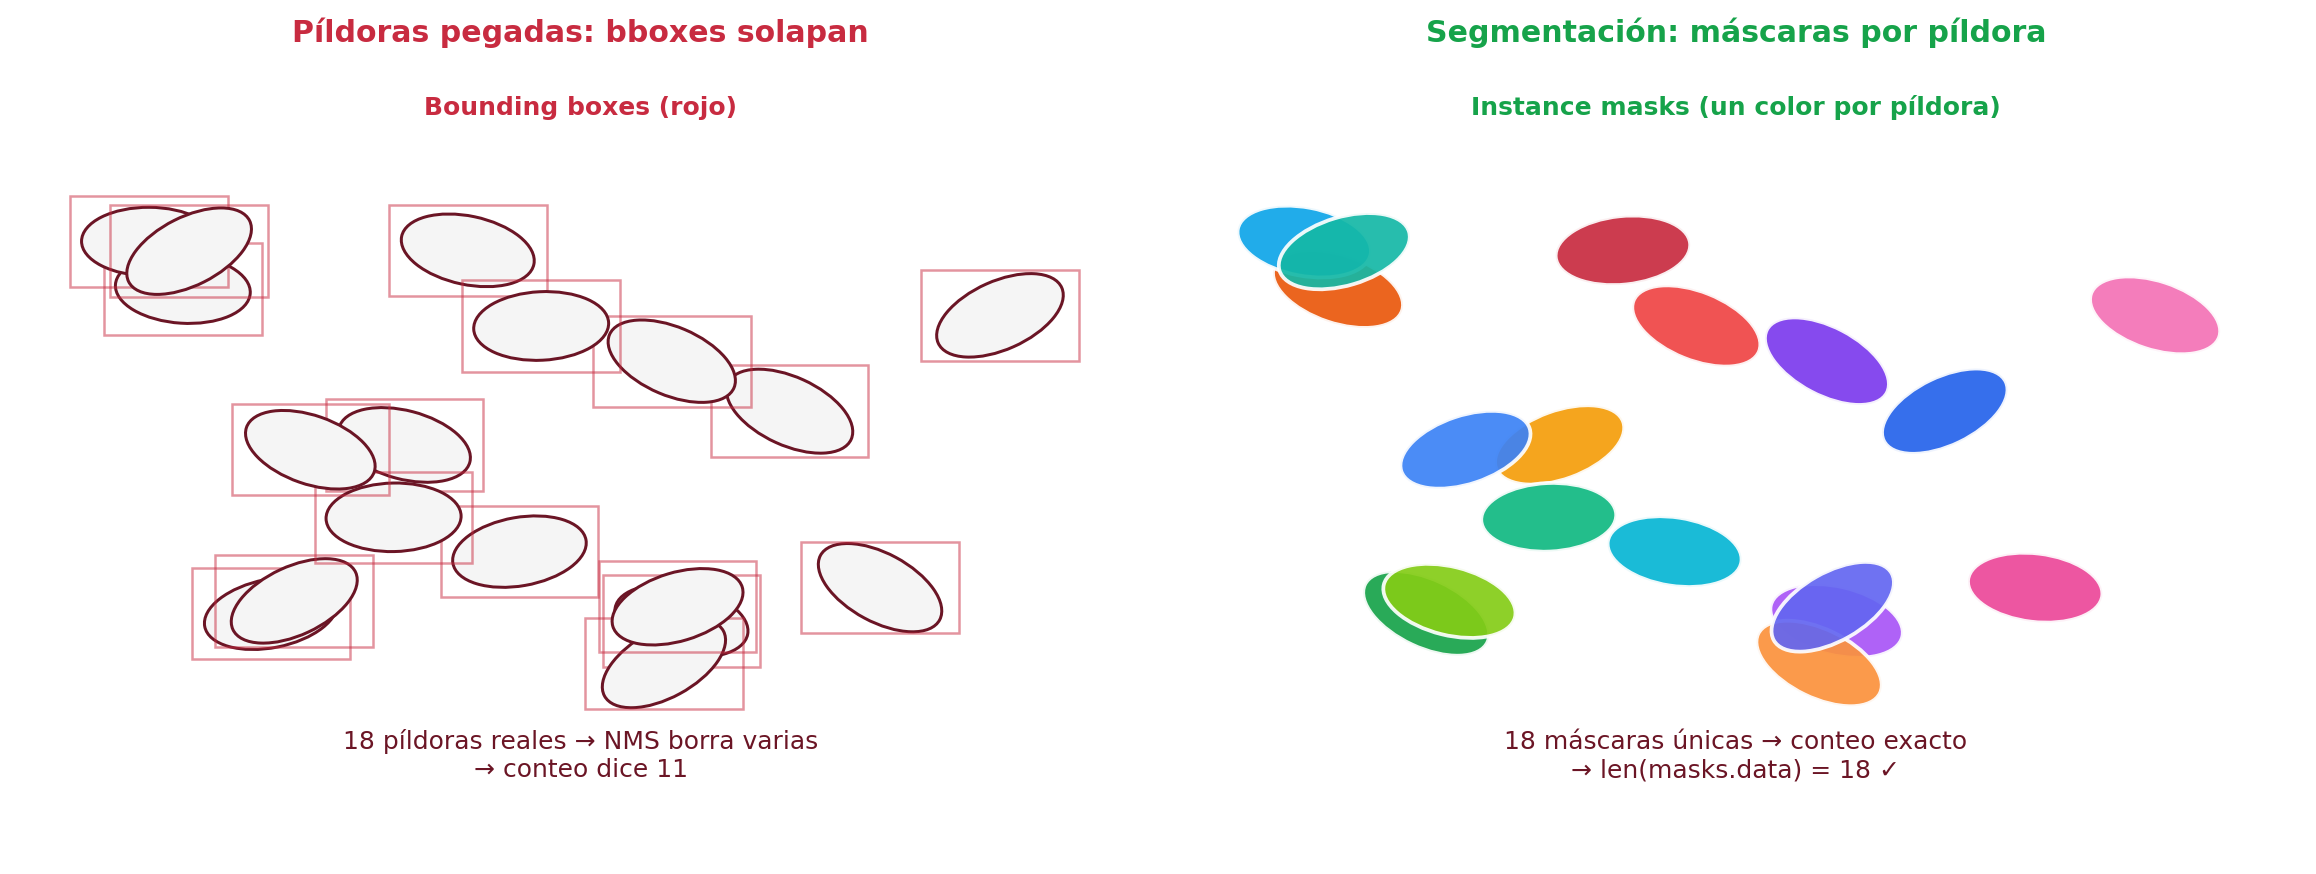
\includegraphics[width=0.97\textwidth]{fig_pills_motivacion.png}
  \end{center}

  \vspace{2pt}
  {\scriptsize\color{textMuted}
    \faLightbulb\hspace{4pt} Cuando los objetos se tocan, las bboxes solapan
    y NMS borra detecciones v\'alidas. Las m\'ascaras a nivel pixel s\'i
    distinguen cada instancia.}
\end{frame}

% =============================================================================
%  BLOQUE 5: API SEGMENTATION
% =============================================================================
\sectionframe{API de Segmentaci\'on}{Mismo objeto YOLO, output enriquecido}

\begin{frame}[fragile,shrink]{Misma API, Solo Cambia el Modelo}
  \vspace{-4pt}
  \begin{pyblock}
from ultralytics import YOLO

# Detection
model = YOLO("yolo26n.pt")
res = model("foto.jpg")[0]
res.boxes               # cajas + clases + conf

# Segmentation
seg_model = YOLO("yolo26n-seg.pt")    # mismo patron, sufijo -seg
res = seg_model("foto.jpg")[0]
res.boxes               # las cajas (siguen estando)
res.masks               # NUEVO: mascaras por objeto

print(f"Detecciones: {len(res.boxes)}")
print(f"Mascaras:    {res.masks.data.shape}")   # (N, H, W) binario
  \end{pyblock}
\end{frame}

\begin{frame}[shrink]{Los 3 Formatos de M\'ascara}
  \vspace{4pt}
  \begin{center}
    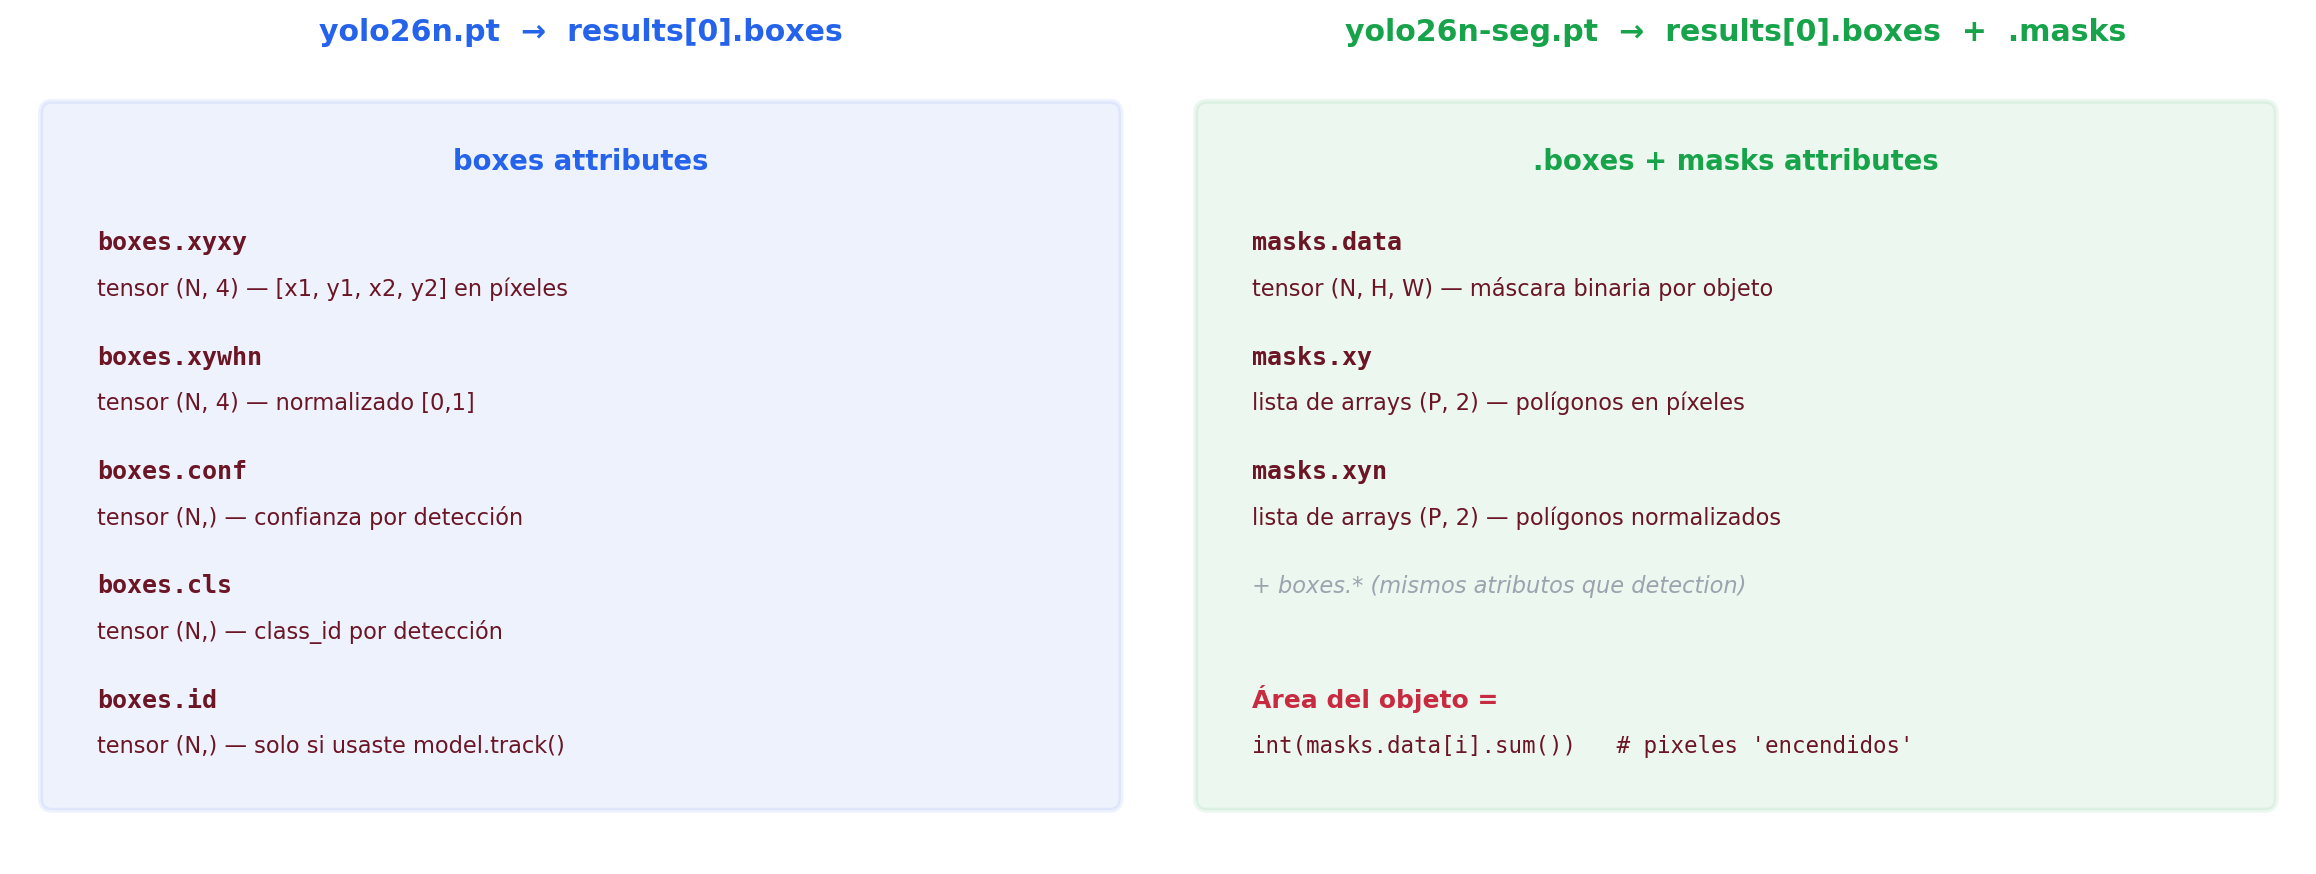
\includegraphics[width=0.97\textwidth]{fig_api_seg.png}
  \end{center}

  \vspace{2pt}
  {\scriptsize\color{textMuted}
    \faLightbulb\hspace{4pt} \texttt{masks.data} para operaciones por pixel
    (\'area, IoU). \texttt{masks.xy} para dibujar. \texttt{masks.xyn} para
    guardar al formato YOLO label.}
\end{frame}

\begin{frame}[fragile,shrink]{Conteo y \'Area en 3 L\'ineas}
  \vspace{-4pt}
  \begin{pyblock}
res = seg_model("blister.jpg", conf=0.25)[0]

# Conteo: cuantas mascaras hay
n_pildoras = len(res.masks.data) if res.masks is not None else 0

# Area de cada una: pixeles "encendidos" en la mascara binaria
for i, mask in enumerate(res.masks.data):
    area = int(mask.sum().item())
    clase = res.names[int(res.boxes.cls[i])]
    conf = float(res.boxes.conf[i])
    print(f"obj {i}: {clase}  conf={conf:.2f}  area={area} px")
  \end{pyblock}

  \vspace{4pt}
  {\scriptsize\color{textMuted}
    \faLightbulb\hspace{4pt} \texttt{mask.sum()} cuenta pixeles 1.
    Filtrar por \'area m\'inima descarta pastillas partidas.}
\end{frame}

% =============================================================================
%  BLOQUE 6: COCO SEG
% =============================================================================
\sectionframe{Clases COCO}{Qu\'e reconoce \texttt{yolo26n-seg} sin entrenar nada}

\begin{frame}[shrink]{Las 80 Clases que Vienen Gratis}
  \vspace{2pt}
  \begin{center}
    
\includegraphics[width=0.96\textwidth]{fig_coco_classes.png}
  \end{center}

  \vspace{2pt}
  {\scriptsize\color{textMuted}
    \faLightbulb\hspace{4pt} Para una demo r\'apida (contar naranjas, personas,
    botellas) no necesitas entrenar. Para algo \emph{tuyo} (p\'ildoras, placas,
    tumores): fine-tune obligatorio.}
\end{frame}

\begin{frame}[fragile,shrink]{Ejemplo: Contar Naranjas Sin Entrenar}
  \vspace{-4pt}
  \begin{pyblock}
seg_model = YOLO("yolo26n-seg.pt")
res = seg_model("bandeja_frutas.jpg", conf=0.25)[0]

# Naranjas = clase 49 en COCO
n_orange = sum(1 for c in res.boxes.cls if int(c) == 49)
print(f"Naranjas detectadas: {n_orange}")

# Filtrar visualizacion solo a naranjas:
res.show(labels=True, conf=True, classes=[49])
  \end{pyblock}

  \vspace{4pt}
  {\scriptsize\color{textMuted}
    \faLightbulb\hspace{4pt} El argumento \texttt{classes=[49]} en
    \texttt{predict} solo evalua esa clase y omite el resto. \'Util para
    pipelines orientados a una categor\'ia espec\'ifica.}
\end{frame}

% =============================================================================
%  BLOQUE 7: PILLS
% =============================================================================
\sectionframe{Caso de Negocio}{Contar p\'ildoras para una farmac\'eutica}

\begin{frame}[shrink]{El Problema}
  \vspace{6pt}
  {\footnotesize\color{arcaDark}\bfseries
    Una farmac\'eutica quiere automatizar el conteo de p\'ildoras en
    bl\'isters durante control de calidad. Una persona cuenta $\sim$600
    p\'ildoras/hora; una c\'amara con visi\'on puede hacer 10.000.}

  \vspace{14pt}
  {\footnotesize
  \begin{itemize}\setlength{\itemsep}{6pt}
    \item[{\color{arcaRed}\scriptsize\faArrowRight}]
      \textbf{Por qu\'e segmentaci\'on:} las p\'ildoras est\'an pegadas en filas;
      bboxes solapan y NMS borra detecciones.
    \item[{\color{arcaRed}\scriptsize\faArrowRight}]
      \textbf{Por qu\'e fine-tune:} COCO no tiene clase \texttt{pill}. El
      modelo pretrained es ciego.
    \item[{\color{arcaRed}\scriptsize\faArrowRight}]
      \textbf{Dataset:} \texttt{pillsegmentation} en Roboflow Universe
      (workspace \texttt{abstract}). $\sim$200 im\'agenes con polígonos.
    \item[{\color{codeGreen}\scriptsize\faArrowRight}]
      \textbf{M\'etrica clave:} mAP@0.5 (mask) + conteo exacto en validation.
  \end{itemize}
  }
\end{frame}

\begin{frame}[shrink]{Pipeline Completo}
  \vspace{2pt}
  \begin{center}
    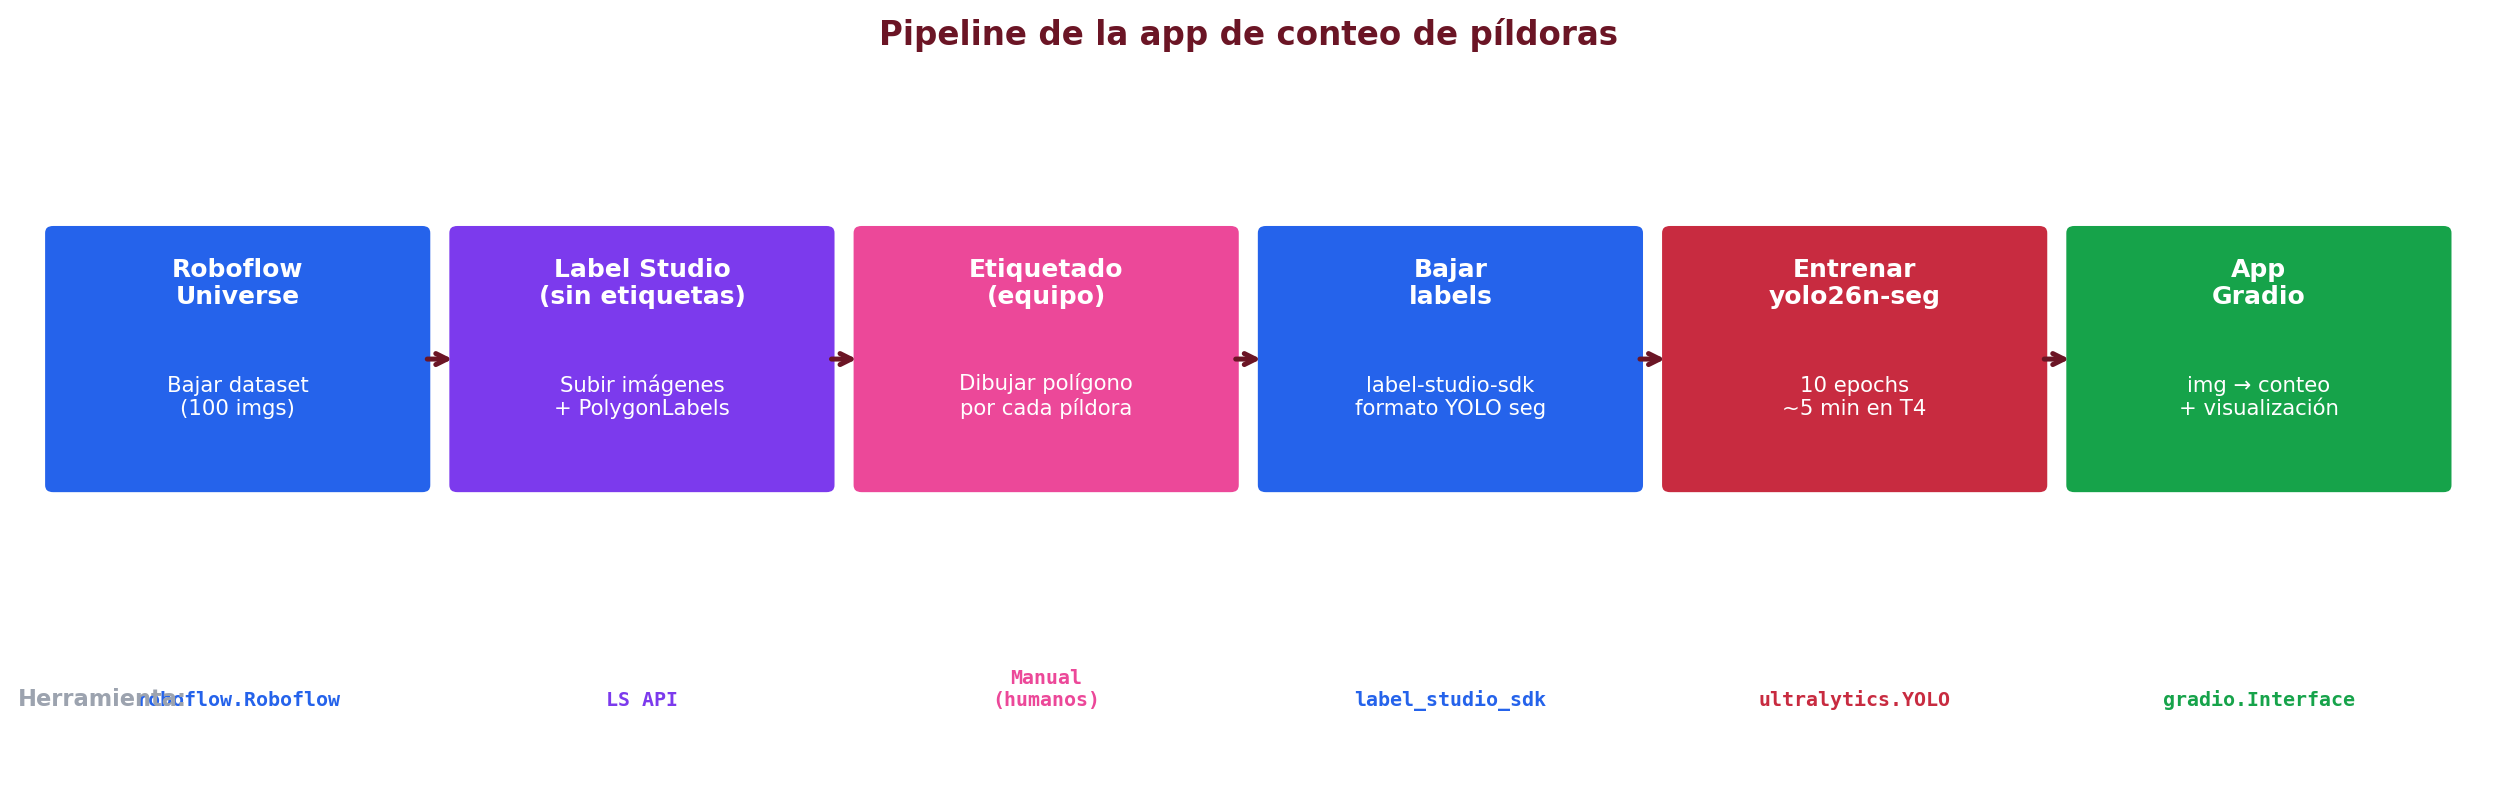
\includegraphics[width=0.97\textwidth]{fig_pill_pipeline.png}
  \end{center}

  \vspace{2pt}
  {\scriptsize\color{textMuted}
    \faLightbulb\hspace{4pt} Roboflow para conseguir datos. LS para que el
    equipo etiquete (pr\'actica). Ultralytics para entrenar. Gradio para
    el producto. Stack de 4 piezas, todo Python.}
\end{frame}

\begin{frame}[fragile,shrink]{Bajar de Roboflow Universe}
  \vspace{-4pt}
  \begin{pyblock}
from roboflow import Roboflow

rf = Roboflow(api_key="DJqoR0JeH6JaOrpH712W")
project = rf.workspace("abstract").project("pillsegmentation-oyygy")

# Ultima version disponible
version = project.versions()[0]

# Baja en formato yolov8 (compatible con yolo26)
dataset = version.download("yolov8", location="pills_raw")
print(f"Bajado en: {dataset.location}")
  \end{pyblock}

  \vspace{4pt}
  {\scriptsize\color{textMuted}
    \faLightbulb\hspace{4pt} Roboflow Universe es como GitHub para datasets
    de visi\'on. Hay 200K+ datasets p\'ublicos, muchos con polígonos
    listos para fine-tune.}
\end{frame}

\begin{frame}[fragile,shrink]{Subir 100 Im\'agenes a LS \emph{sin} Etiquetas}
  \vspace{-4pt}
  \begin{pyblock}
# El profesor corrio setup_labelstudio.py con:
#   - 100 imagenes al azar del dataset Roboflow
#   - PolygonLabels (no RectangleLabels!)
#   - Sin annotations: las hacen ustedes

LABELING_CONFIG = """
<View>
  <Image name="image" value="$image"/>
  <PolygonLabels name="label" toName="image">
    <Label value="pill" background="#C82B40"/>
  </PolygonLabels>
</View>
"""

# Tarea (15 min en clase): cada uno etiqueta al menos 5 imagenes.
  \end{pyblock}

  \vspace{4pt}
  {\scriptsize\color{textMuted}
    \faLightbulb\hspace{4pt} En LS, tecla \texttt{Z} cierra el pol\'igono.
    Una p\'ildora $=$ un pol\'igono. P\'ildoras pegadas $=$ dos pol\'igonos
    separados (eso es justamente lo que el modelo va a aprender).}
\end{frame}

\begin{frame}[fragile,shrink]{Entrenar \texttt{yolo26n-seg}}
  \vspace{-4pt}
  \begin{pyblock}
from ultralytics import YOLO

# Mismo patron, modelo con sufijo -seg
seg_model = YOLO("yolo26n-seg.pt")

results = seg_model.train(
    data=str(yaml_path_pills),
    epochs=20,
    imgsz=640,
    batch=8,
    device="cuda",
    project="runs", name="pills",
)

# Validar - dos juegos de metricas
m = seg_model.val()
print(f"BBox mAP@0.5 = {m.box.map50:.3f}")
print(f"Mask mAP@0.5 = {m.seg.map50:.3f}")   # la que importa
  \end{pyblock}
\end{frame}

% =============================================================================
%  BLOQUE 8: APP GRADIO
% =============================================================================
\sectionframe{App Gradio}{El modelo entrenado se vuelve un producto}

\begin{frame}[shrink]{La App que Vamos a Construir}
  \vspace{2pt}
  \begin{center}
    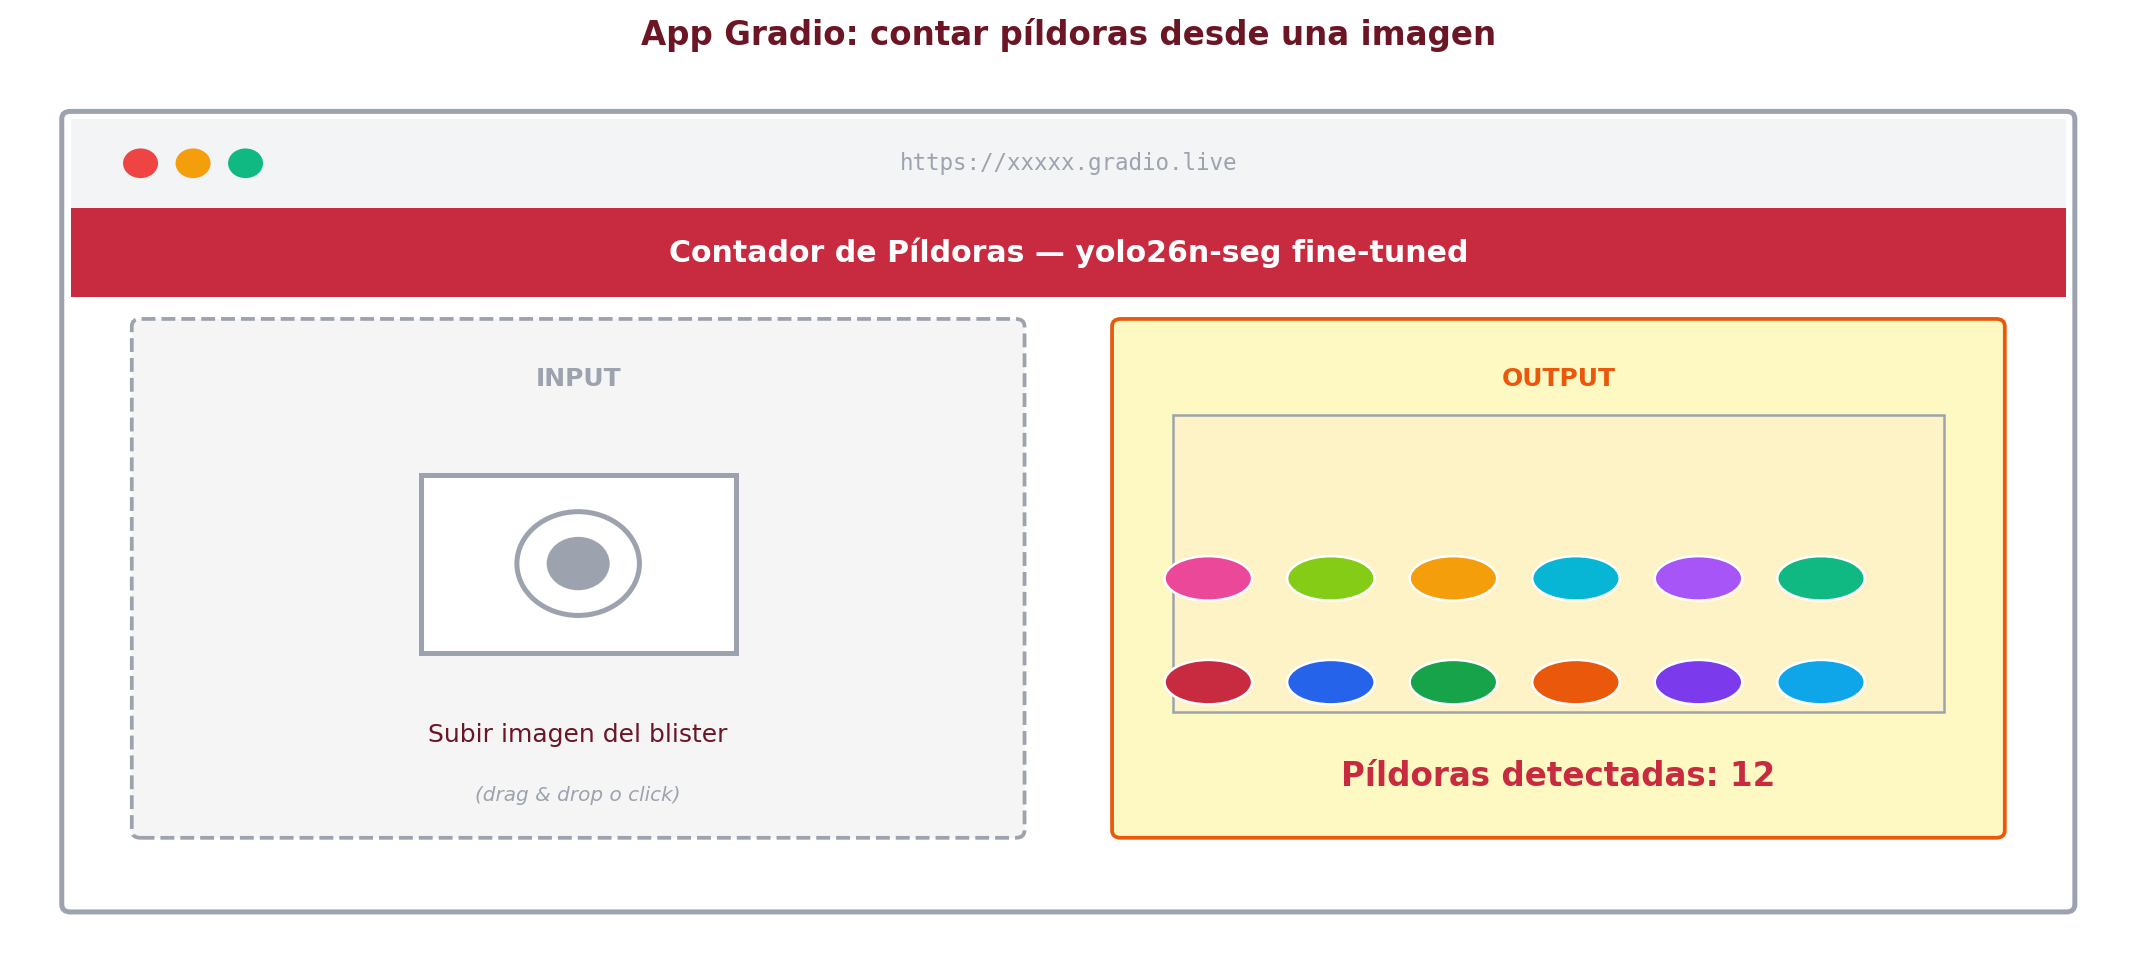
\includegraphics[width=0.85\textwidth]{fig_gradio_mockup.png}
  \end{center}

  \vspace{2pt}
  {\scriptsize\color{textMuted}
    \faLightbulb\hspace{4pt} Gradio convierte una funci\'on Python en una
    mini-app web con sliders y upload. Ideal para validar con stakeholders
    antes de invertir en una API "de verdad".}
\end{frame}

\begin{frame}[fragile,shrink]{C\'odigo Completo de la App}
  \vspace{-4pt}
  \begin{pyblock}
import gradio as gr

modelo = YOLO("models/pills_yolo26n-seg_2026-05-15.pt")

def contar(imagen, conf, area_min):
    res = modelo(imagen, conf=conf)[0]
    if res.masks is None:
        return imagen, "Sin detecciones"
    areas = res.masks.data.sum(dim=(1, 2)).cpu().numpy()
    n_total = len(areas)
    n_validas = int((areas >= area_min).sum())
    return res.plot()[..., ::-1], f"Pildoras: {n_total} (enteras: {n_validas})"

gr.Interface(
    fn=contar,
    inputs=[gr.Image(type="numpy"),
            gr.Slider(0.1, 0.9, value=0.25, label="Confianza"),
            gr.Slider(100, 2000, value=500, label="Area minima")],
    outputs=[gr.Image(), gr.Textbox()],
).launch(share=True)
  \end{pyblock}
\end{frame}

% =============================================================================
%  BLOQUE 9: CIERRE
% =============================================================================
\sectionframe{Cierre}{Lo que aprendimos hoy y la tarea}

\begin{frame}[shrink]{Resumen}
  \vspace{6pt}
  \begin{columns}[T]
    \begin{column}{0.48\textwidth}
      {\footnotesize\bfseries\color{arcaDark} El stack:}
      \vspace{4pt}

      {\scriptsize
      \begin{itemize}\setlength{\itemsep}{4pt}
        \item \textbf{Roboflow Universe} para conseguir datasets.
        \item \textbf{Label Studio} para etiquetar pol\'igonos.
        \item \textbf{Ultralytics YOLO} para entrenar (sufijo \texttt{-seg}).
        \item \textbf{Gradio} para el producto final.
      \end{itemize}
      }
    \end{column}
    \begin{column}{0.48\textwidth}
      {\footnotesize\bfseries\color{arcaDark} Las lecciones:}
      \vspace{4pt}

      {\scriptsize
      \begin{itemize}\setlength{\itemsep}{4pt}
        \item \textbf{La m\'etrica la decide el dominio.} Precision para LPR,
              recall para tumor, F1 para p\'ildoras.
        \item \textbf{\texttt{best.pt}} es lo \'unico que viaja a producci\'on.
        \item \textbf{Segmentation = conteo robusto.} Bboxes pierden cuando los
              objetos se pegan.
        \item \textbf{COCO ya cuenta} naranjas, personas, botellas. Solo entrenas
              cuando tu clase no est\'a.
      \end{itemize}
      }
    \end{column}
  \end{columns}

  \vspace{12pt}
  \begin{tcolorbox}[colback=codeGreen!8, colframe=codeGreen, boxrule=0.5pt,
    arc=2pt, left=6pt, right=6pt, top=4pt, bottom=4pt]
    {\scriptsize\color{arcaDark}
    \faKey\hspace{4pt}\textbf{Tarea:} (1) etiquetar al menos 10 im\'agenes de
    p\'ildoras en LS. (2) Re-entrenar con \emph{sus} etiquetas. (3) Probar
    la app Gradio con una foto propia (monedas, granos, frutas, lo que
    sea contable). Traer un screenshot del conteo.}
  \end{tcolorbox}
\end{frame}

% ── QR DE CIERRE ──────────────────────────────────────────────────────
{
\setbeamertemplate{headline}{}
\setbeamertemplate{footline}{}
\begin{frame}[plain, noframenumbering]
  \begin{tikzpicture}[remember picture, overlay]
    \fill[arcaDark] (current page.south west) rectangle (current page.north east);
  \end{tikzpicture}
  \vspace{1.0cm}
  \begin{center}
    {\color{white}\Huge\bfseries Encuesta de Cierre} \\[0.4cm]
    {\color{white!85}\Large Cu\'entanos qu\'e tal estuvo la clase}
    \vspace{1cm}

    
\includegraphics[width=4.5cm]{qr_encuesta.jpg}

    \vspace{0.6cm}
    {\color{white!80}\small Gracias por hoy --- nos vemos la pr\'oxima}
  \end{center}
\end{frame}
}

\end{document}
